\documentclass[11pt,a4paper]{article}
\usepackage[utf8]{inputenc}
\usepackage[T1]{fontenc}
\usepackage[spanish]{babel}
\usepackage{geometry}
\usepackage{graphicx}
\usepackage{booktabs}
\usepackage{tabularx}
\usepackage[table]{xcolor}
\usepackage{enumitem}
\usepackage{hyperref}
\usepackage{fancyhdr}
\geometry{margin=18mm}
\hypersetup{colorlinks=true,linkcolor=blue,urlcolor=blue}
\pagestyle{fancy}\fancyhf{}
\setlength{\headheight}{14pt}
\lhead{Nova Spot Micro 3}\rhead{Conexiones electrónicas}\cfoot{\thepage}
\newcommand{\ok}{\textcolor{green!45!black}{\textbf{Confirmado en diseño}}}
\newcommand{\pending}{\textcolor{orange!80!black}{\textbf{Pendiente de verificar}}}
\newcommand{\blocked}{\textcolor{red!75!black}{\textbf{No energizar}}}
\newcommand{\code}[1]{\texttt{#1}}

\begin{document}

\begin{center}
{\LARGE\bfseries Nova Spot Micro 3\\[2mm]
Guía de conexiones para Raspberry, PCA9685, servos y sensores}\par
\vspace{3mm}
{\large Documento de montaje progresivo --- 17 de agosto de 2026}
\end{center}

\begin{center}
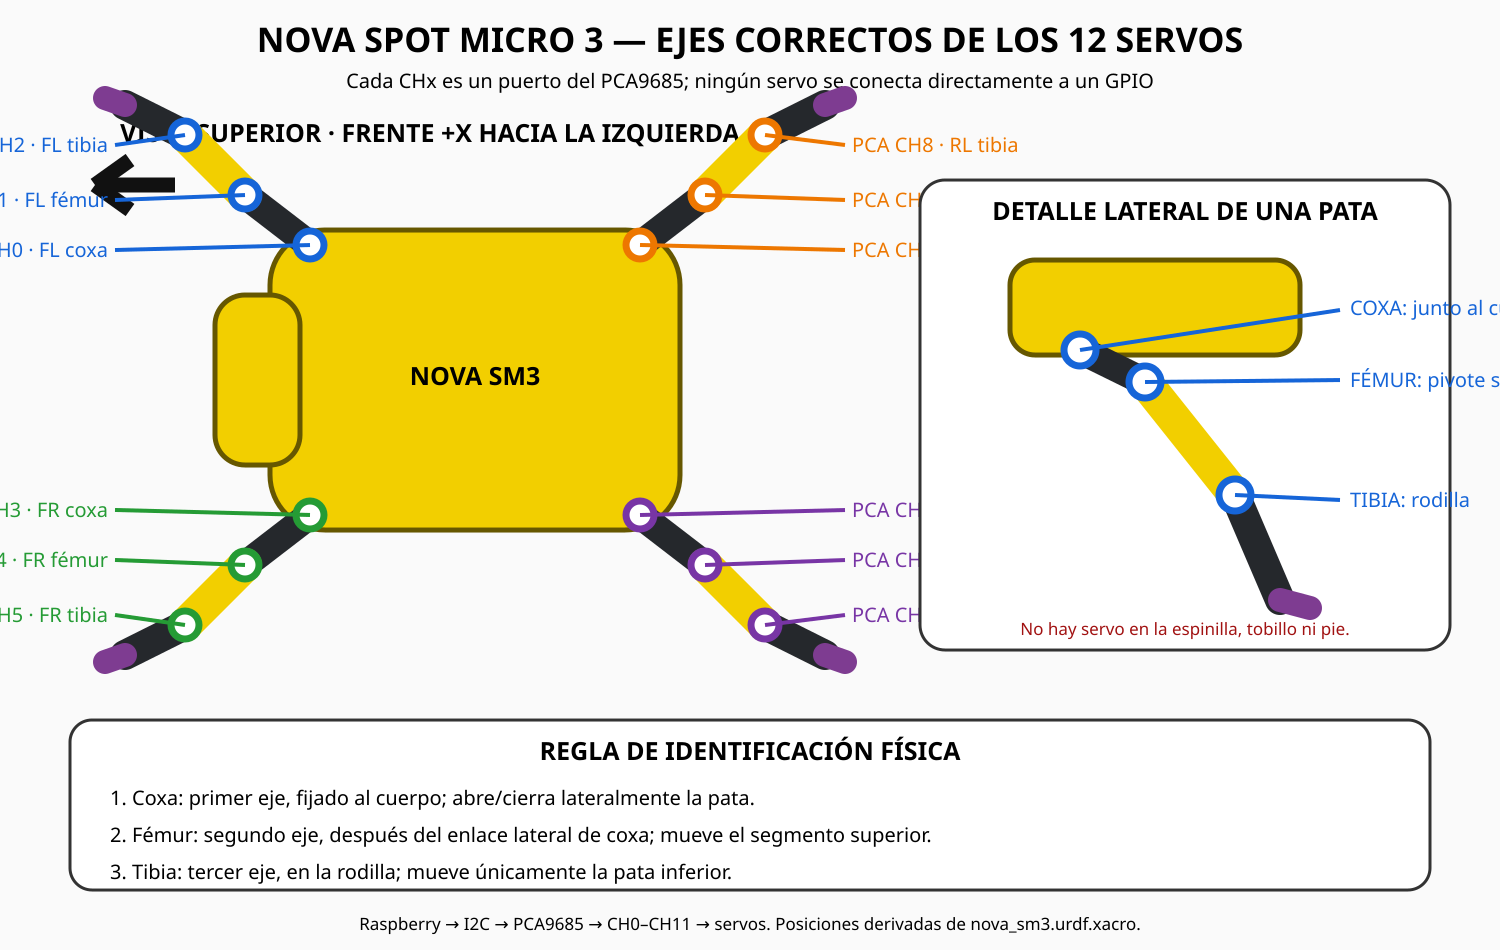
\includegraphics[width=0.94\textwidth]{../mapa_articulaciones_novasm3_corregido.png}
\end{center}

\begin{tabularx}{\textwidth}{>{\bfseries}l X}
Propósito & Identificar qué componente se conecta a cada pin y qué servo ocupa cada canal del PCA9685.\\
Alcance & Raspberry Pi, PCA9685, doce servos, BNO055 y DS18B20 propuestos, potencia y seguridad.\\
Limitación & No sustituye la calibración eléctrica ni autoriza conectar simultáneamente los doce servos.\\
\end{tabularx}

\vfill
\begin{center}
\fcolorbox{red!70!black}{red!5}{\parbox{0.9\textwidth}{\centering\bfseries
Los servos NO se conectan directamente a los GPIO de la Raspberry.\\
Raspberry $\rightarrow$ I2C $\rightarrow$ PCA9685 $\rightarrow$ CH0--CH11 $\rightarrow$ servos.}}
\end{center}

\newpage
\section{Inventario y estado real}

\begin{tabularx}{\textwidth}{l c X l}
\toprule
\textbf{Elemento} & \textbf{Cantidad} & \textbf{Función} & \textbf{Estado}\\
\midrule
Raspberry Pi & 1 & Ejecuta ROS 2, marcha, seguridad y registro. El seguimiento menciona Pi 3/3B+; el presupuesto menciona Pi 5. & \pending\\
PCA9685 & 1 & Genera 16 PWM por I2C; se usarán CH0--CH11. & \ok\\
Servomotores MG996R & 12 & Tres articulaciones por pata. Marca/modelo de cada unidad debe confirmarse. & \pending\\
BNO055 & 1 & Orientación e IMU por I2C. Aparece en presupuesto, no confirmado físicamente. & \pending\\
DS18B20 & 12 & Temperatura por bus 1-Wire. Cantidad y necesidad deben confirmarse. & \pending\\
LM2596 ajustable & 1 & Regulación DC-DC. Capacidad térmica/corriente no validada para doce servos. & \blocked\\
Fuente, fusible e interruptor & Por definir & Potencia de servos y corte físico de emergencia. & \blocked\\
PCB, headers y conectores & Por confirmar & Distribución y montaje. & \pending\\
\bottomrule
\end{tabularx}

\subsection{Arquitectura eléctrica}

\begin{enumerate}[leftmargin=8mm]
\item La Raspberry alimenta únicamente la \textbf{lógica} del PCA9685 con 3,3 V.
\item SDA y SCL transportan las órdenes I2C; no llevan potencia de motores.
\item Una fuente externa regulada alimenta \code{V+} y los doce servos.
\item Todas las tierras se unen en un punto controlado: Raspberry, PCA9685 y fuente externa.
\item El pin \code{OE} mantiene las salidas apagadas durante arranque, error o parada.
\end{enumerate}

\begin{center}
\fcolorbox{orange!80!black}{orange!8}{\parbox{0.9\textwidth}{
\textbf{Contradicción por resolver:} confirmar físicamente si el computador disponible es Raspberry Pi 3B/3B+ o Raspberry Pi 5. El conector principal de 40 pines conserva SDA1/SCL1 en los pines físicos 3 y 5, pero el documento final debe registrar el modelo exacto.}}
\end{center}

\newpage
\section{Pines Raspberry hacia PCA9685}

\begin{tabularx}{\textwidth}{c l l X}
\toprule
\textbf{Pin físico} & \textbf{Raspberry/BCM} & \textbf{PCA9685} & \textbf{Función}\\
\midrule
1 & 3V3 & VCC & Lógica a 3,3 V; no es potencia de servos.\\
3 & GPIO2 / SDA1 & SDA & Datos del bus I2C.\\
5 & GPIO3 / SCL1 & SCL & Reloj del bus I2C.\\
6 & GND & GND & Referencia común de lógica y potencia.\\
11 & GPIO17 & OE & Activo en bajo: LOW habilita; HIGH apaga PWM.\\
\bottomrule
\end{tabularx}

\subsection{Conexión de seguridad de OE}

\begin{itemize}[leftmargin=7mm]
\item Colocar resistencia \textbf{pull-up de 10 k$\Omega$} entre OE y 3,3 V.
\item GPIO17 controla OE, pero la resistencia garantiza apagado durante el arranque.
\item La parada física debe cortar o deshabilitar potencia aunque ROS 2 falle.
\end{itemize}

\subsection{Conector de cada servo}

\begin{tabularx}{\textwidth}{l l X}
\toprule
\textbf{Color habitual} & \textbf{PCA9685} & \textbf{Conexión}\\
\midrule
Marrón o negro & GND & Retorno común. Confirmar colores del fabricante.\\
Rojo & V+ & Fuente externa regulada de servos, nunca 3V3/VCC.\\
Naranja, amarillo o blanco & PWM & Señal del canal CH0--CH11 correspondiente.\\
\bottomrule
\end{tabularx}

\begin{center}
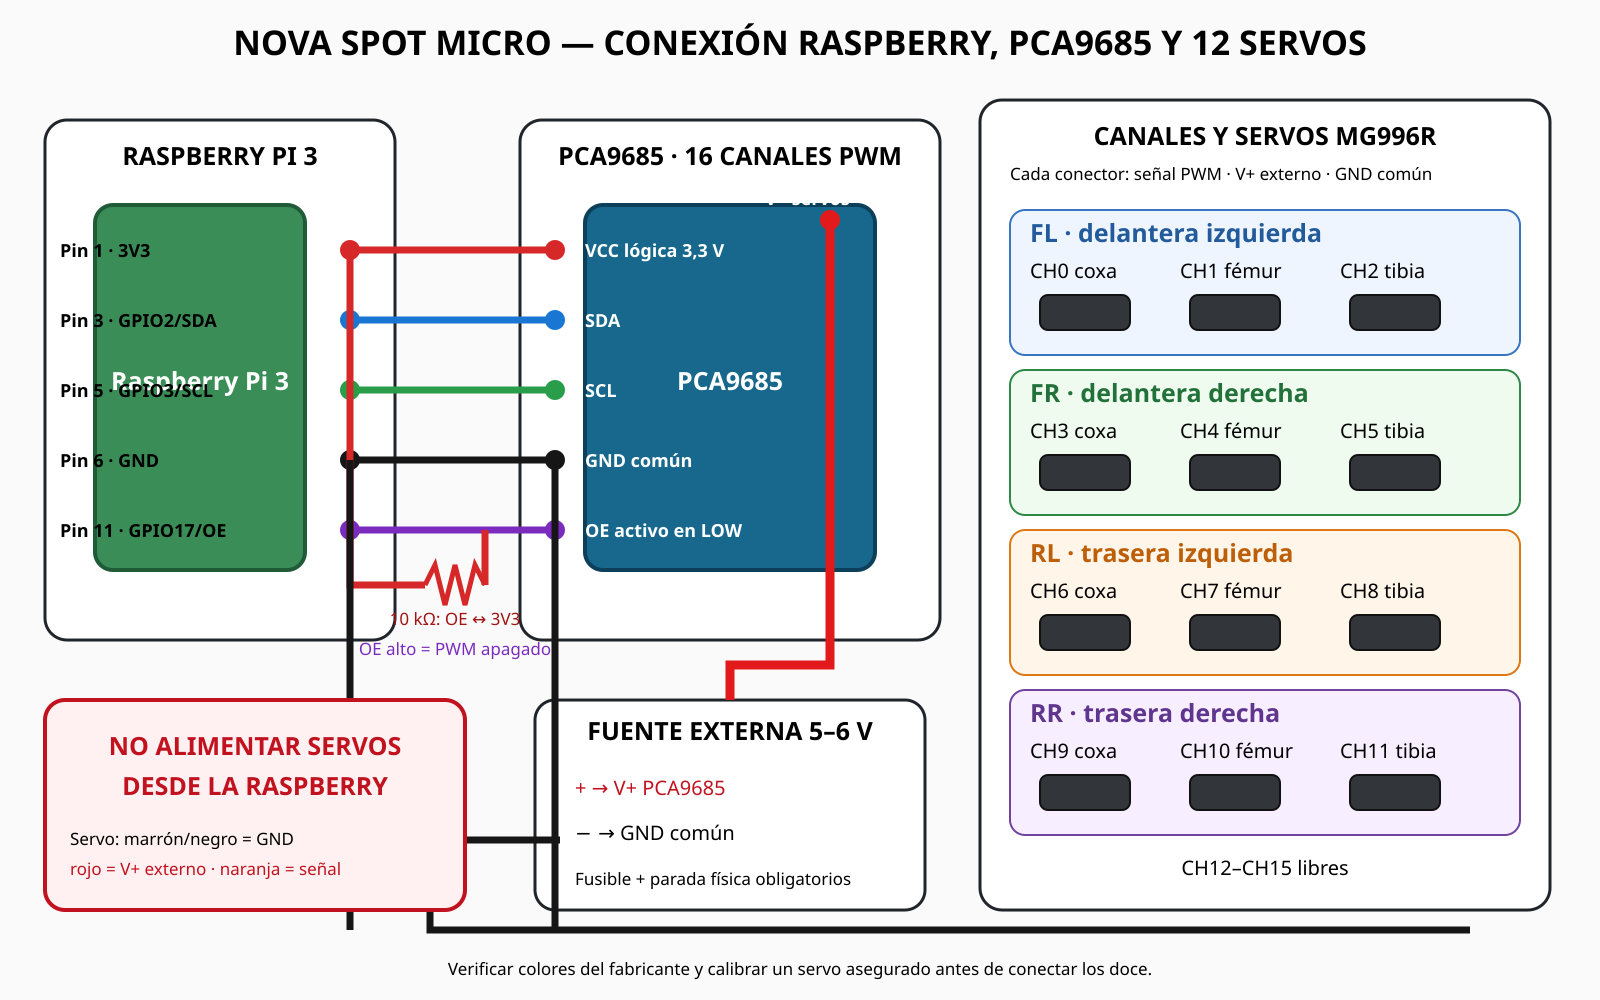
\includegraphics[width=0.98\textwidth]{../diagrama_conexion_servos.png}
\end{center}

\newpage
\section{Mapa de los doce servos}

\begin{tabularx}{\textwidth}{c l l X}
\toprule
\textbf{Canal PCA} & \textbf{Pata} & \textbf{Articulación} & \textbf{Nombre ROS 2}\\
\midrule
CH0 & FL, delantera izquierda & Coxa & \code{front\_left\_coxa\_joint}\\
CH1 & FL & Fémur & \code{front\_left\_femur\_joint}\\
CH2 & FL & Tibia/rodilla & \code{front\_left\_tibia\_joint}\\
CH3 & FR, delantera derecha & Coxa & \code{front\_right\_coxa\_joint}\\
CH4 & FR & Fémur & \code{front\_right\_femur\_joint}\\
CH5 & FR & Tibia/rodilla & \code{front\_right\_tibia\_joint}\\
CH6 & RL, trasera izquierda & Coxa & \code{rear\_left\_coxa\_joint}\\
CH7 & RL & Fémur & \code{rear\_left\_femur\_joint}\\
CH8 & RL & Tibia/rodilla & \code{rear\_left\_tibia\_joint}\\
CH9 & RR, trasera derecha & Coxa & \code{rear\_right\_coxa\_joint}\\
CH10 & RR & Fémur & \code{rear\_right\_femur\_joint}\\
CH11 & RR & Tibia/rodilla & \code{rear\_right\_tibia\_joint}\\
\bottomrule
\end{tabularx}

\begin{center}
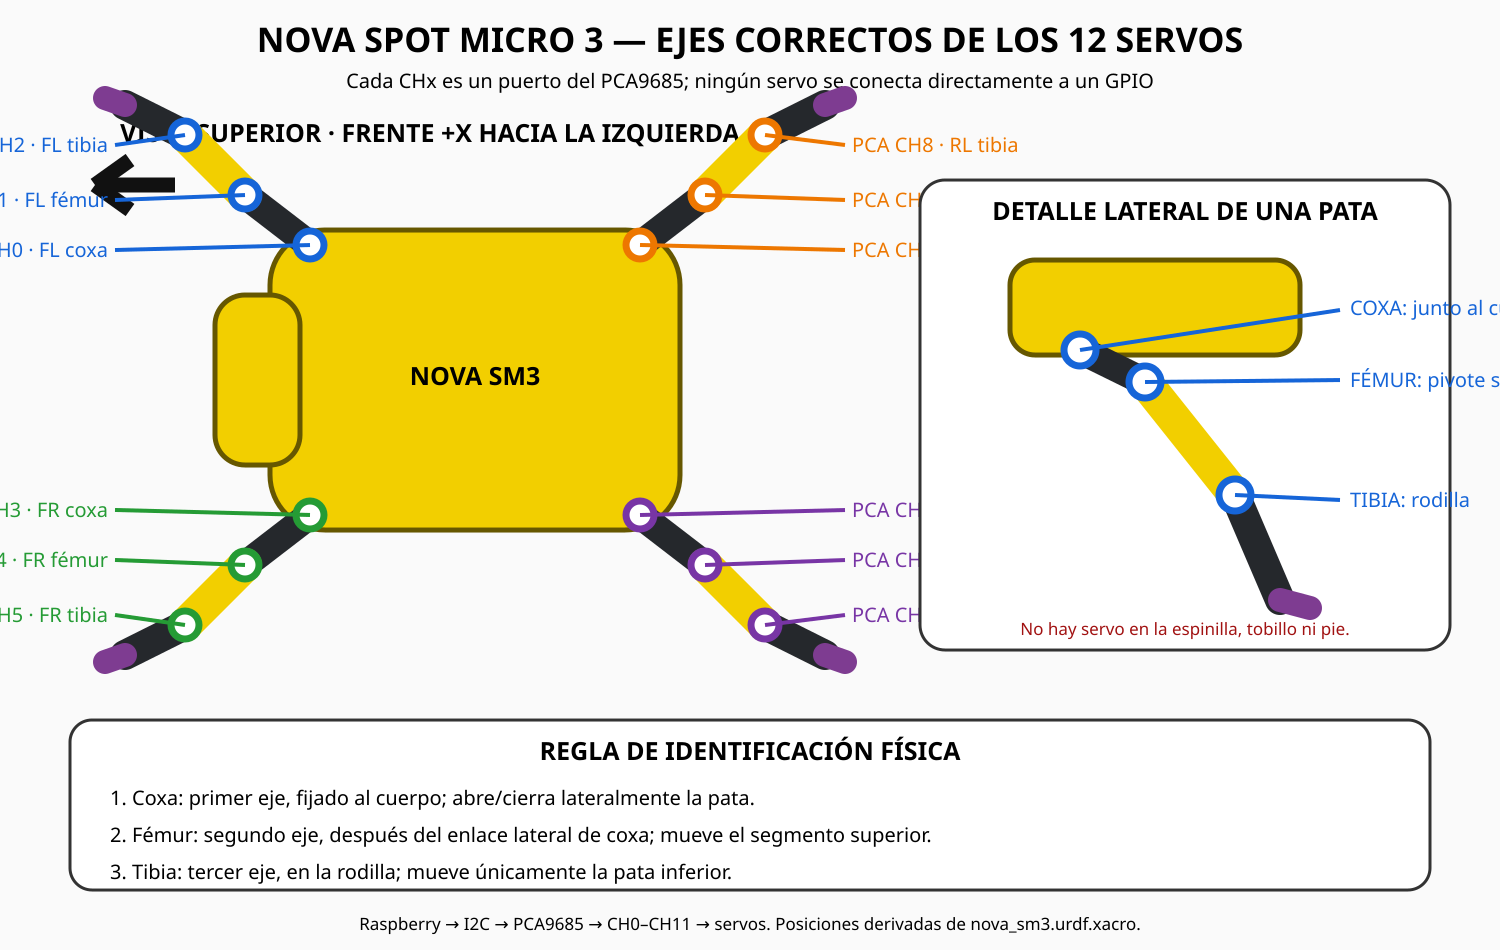
\includegraphics[width=0.96\textwidth]{../mapa_articulaciones_novasm3_corregido.png}
\end{center}

\textbf{Regla física:} coxa está junto al cuerpo; fémur es el segundo eje superior; tibia está en la rodilla. No existe un servo adicional en espinilla, tobillo o pie.

\newpage
\section{Sensores y otros materiales propuestos}

Estas conexiones son una \textbf{propuesta de integración}; deben confirmarse después de identificar el módulo exacto y sus niveles eléctricos.

\subsection{BNO055 por el mismo bus I2C}

\begin{tabularx}{\textwidth}{c l l X}
\toprule
\textbf{Pin físico} & \textbf{Raspberry} & \textbf{BNO055} & \textbf{Observación}\\
\midrule
1 & 3V3 & VIN/VCC & Solo si el módulo identificado acepta 3,3 V.\\
3 & GPIO2/SDA1 & SDA & Compartido con PCA9685.\\
5 & GPIO3/SCL1 & SCL & Compartido con PCA9685.\\
6 & GND & GND & Tierra común.\\
\bottomrule
\end{tabularx}

Antes de conectarlo: revisar serigrafía, dirección I2C y regulador del breakout. No asumir que todos los módulos BNO055 tienen el mismo pinout.

\subsection{DS18B20 por bus 1-Wire}

\begin{tabularx}{\textwidth}{c l l X}
\toprule
\textbf{Pin físico} & \textbf{Raspberry} & \textbf{DS18B20} & \textbf{Observación}\\
\midrule
1 & 3V3 & VDD & Alimentación de sensores.\\
7 & GPIO4 & DQ & Bus de datos compartido; pull-up de 4,7 k$\Omega$ a 3,3 V.\\
6 & GND & GND & Tierra común.\\
\bottomrule
\end{tabularx}

Los doce sensores, si realmente se adoptan, se conectan en paralelo al mismo bus y se identifican por su dirección única. Confirmar primero si la medición individual de doce temperaturas aporta valor experimental.

\subsection{LM2596, fuente y potencia}

\begin{itemize}[leftmargin=7mm]
\item El LM2596 no queda aprobado automáticamente como fuente de doce MG996R.
\item Ajustar la salida con multímetro \textbf{sin servos conectados}.
\item Dimensionar fuente, regulador, fusible, cables y conectores usando corriente medida de un servo asegurado y escenarios de arranque/bloqueo.
\item Mantener potencia de servos separada de la alimentación de la Raspberry.
\end{itemize}

\newpage
\section{Orden obligatorio de puesta en marcha}

\begin{enumerate}[leftmargin=8mm]
\item Confirmar inventario: modelo de Raspberry, módulo PCA9685, doce servos y sensores disponibles.
\item Montar Raspberry--PCA9685 con \code{V+} desconectado y OE mantenido en HIGH.
\item Verificar I2C con \code{i2cdetect -y 1}; dirección esperada usual del PCA9685: \code{0x40}, pero debe observarse realmente.
\item Comprobar PWM CH0 con osciloscopio o analizador, sin servo.
\item Medir y registrar un servo asegurado: centro, sentido, mínimo, máximo, velocidad, corriente y temperatura.
\item Conectar un solo servo y mantener la articulación libre de topes.
\item Repetir la calibración para CH0--CH11 en \code{configuracion/servos.yaml}.
\item Probar una pata suspendida, luego cuatro patas con el robot suspendido.
\item Solo después probar postura con soporte, parada física accesible y límite de corriente.
\item Ejecutar un paso, un ciclo y finalmente marcha continua con registro.
\end{enumerate}

\section{Relación con Thonny y Gazebo}

\begin{center}
\fbox{\parbox{0.92\textwidth}{\centering
\code{gait\_controller} $\rightarrow$ trayectoria articular $\rightarrow$
\code{interfaz\_pwm\_ros2.py} $\rightarrow$ calibración $\rightarrow$
PCA9685 $\rightarrow$ MG996R}}
\end{center}

Gazebo y el robot físico usan las mismas referencias articulares, pero la equivalencia depende de medir centro, dirección, límites y velocidad de cada servo. El MG996R recibe posición por PWM; el torque no se ordena directamente y debe estimarse o medirse.

\subsection{Archivos asociados}

\begin{itemize}
\item \code{Raspberry/codigo/interfaz\_pwm\_ros2.py}
\item \code{Raspberry/codigo/pca9685\_seguro.py}
\item \code{Raspberry/configuracion/servos.yaml}
\item \code{Raspberry/configuracion/calibracion\_servos.csv}
\item \code{Raspberry/CONEXIONES.md}
\end{itemize}

\vfill
\begin{center}
\blocked\ hasta completar seguridad eléctrica y calibración individual.
\end{center}

\end{document}
